\graphicspath{{./Ch3-CNN/images/}}

\chapter{Optimizing the Performance of CNN Accelerators} \label{chap:CNN}
CNNs are the state of the art machine learning algorithms. CNNs can achieve human-like accuracy in computer vision-related tasks. In order to achieve high accuracy, modern CNNs use deep hierarchy of layers and perform compute-intensive and memory-intensive operations. CNN accelerators use many processing elements to exploit parallelism to speed up the computations. However, limited off-chip memory bandwidth limits their performance. In addition, considerable data transfer volume from the off-chip memory also results in high energy consumption.

CNNs have a sequence of mainly three types of layers: convolution layer (CL), pooling layer, and fully connected layer (FCL). There are several CLs, and a pooling layer usually follows each CL. The last few layers of the CNNs are FCLs. VGG16 has thirteen CLs and last three layers are FC. Similarly, AlexNet has five CLs, followed by 3 FCLs. Each CL and FCL layer takes 3D input frames (\textit{ifm}) and applies filter weights (\textit{wts}) to compute output frames (\textit{ofm}). Pooling layer computations involve sliding a two dimensional filter window over a single channel of \textit{ifm} and selecting one activation from the window using an operation like maximum or average. There are no parameters in pooling layers. Pooling layer helps in reducing the activation sizes and thus the number of parameters in subsequent layers. CL and FC layer computations involve several parameters. The computations of a CL and an FCL are illustrated in Figure~\ref{fig:CLOps} and~\ref{fig:FCLOps}, respectively. 
\begin{figure}[!htb]
	\centering
	\captionsetup{font=sf}	
	\subfloat[Convolution Layer]{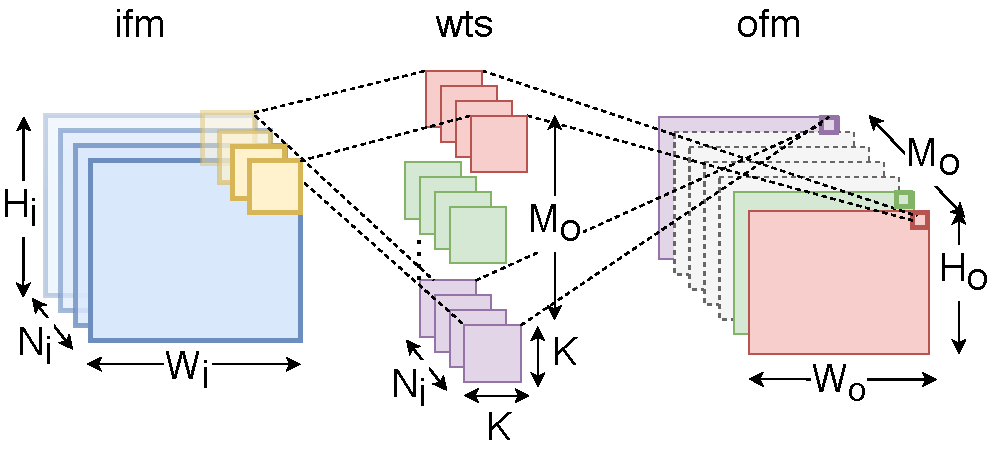
\includegraphics[width=0.49\textwidth]{CLOps.pdf}
		\label{fig:CLOps}}
	\hfil	
	\subfloat[Fully Connected Layer]{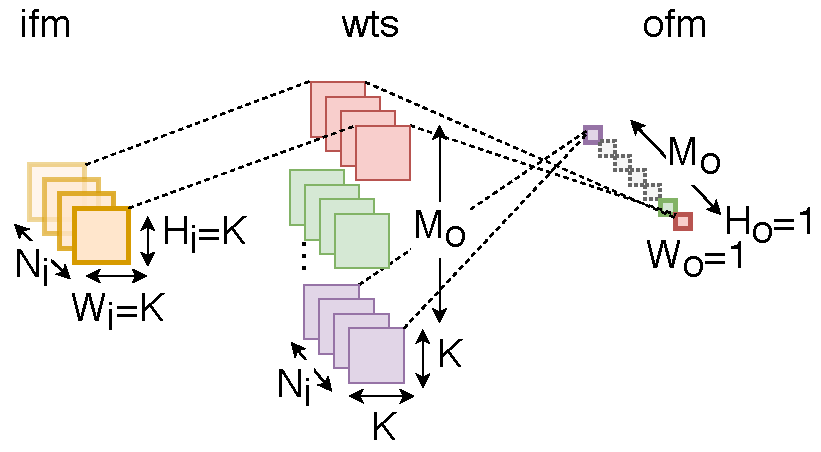
\includegraphics[width=0.42\textwidth]{FCLOps.pdf}
		\label{fig:FCLOps}}
	\hfil	
	\caption{Convolution and fully connected layers}
	\label{fig:CNNAcceleratorAndCLOps}
\end{figure}

CNN accelerators have limited on-chip memory size. Layer activations and parameters sizes are too large to fit into the on-chip memory. To peform the computations CNN accelerators apply loop tiling to partition the layer data into small tiles that fit into on-chip memory. Loop tiling is a compiler  technique~\cite{aho2006compilers} that partitions the loop iteration space and large arrays into smaller tiles to increase the data locality and ensures that data fits into smaller memories. Fig.~\ref{fig:partitioningDataUsingTiling} shows a layer's data stored in off-chip memory and its tiles in the accelerator's on-chip buffer.
\begin{figure}[!htb]
	\centering
	\captionsetup{font=sf}	
	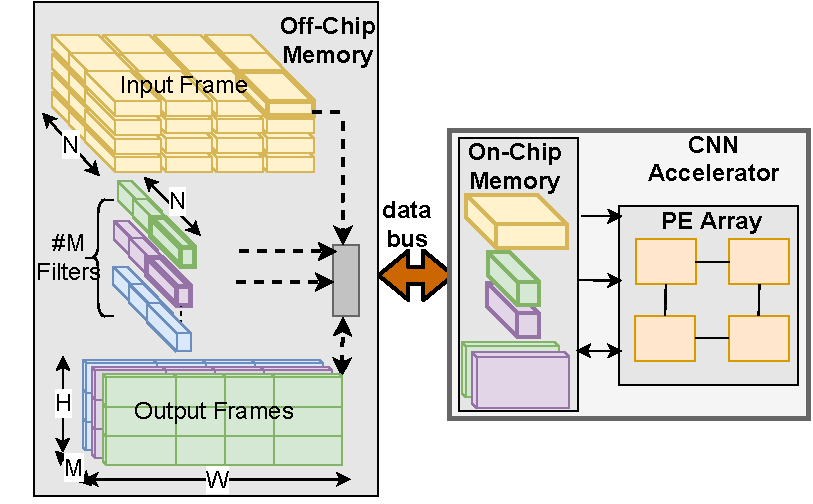
\includegraphics[width=0.5\textwidth]{AboutTheCNNTiles.pdf}
	\caption{CNN layer tiles in off-chip and on-chip memory}
	\label{fig:partitioningDataUsingTiling}
\end{figure}

Pseudo code of tiled version of a convolution layer is shown in Listing~\ref{code:CNNTiledCode}. The outer 5 loops labelled as $L_D,L_H,L_W,L_M,L_N$ selects the tiles of the data and inner loops perform computations on the selected tiles. Order of the outer loops decide the sequence in which different tiles of data are processed. Each of the $5!$ permutations of the outer loop results in a valid schedule. 
%\begin{minipage}{0.9\columnwidth}
\begin{lstlisting}[float,language=C,label=code:CNNTiledCode,caption=Pseudo code of a tiled convolution layer,captionpos=b,belowskip=-1 \baselineskip]
	L_D:for(d=0;d<D;d++) {
		L_H: for(row=0;row<H;row+=Tr) {
			L_W:  for(col=0;col<W;col+=Tc) {
				L_N:  for(ti=0;ti<N;ti+=Tn) {
					L_M:  for(to=0;to<M;to+=Tm) {
						//load wts tile
						//load ifm tile
						//load ofm tile
						for(trr=row;trr<min(row+Tr,H);trr++) {
							for(tcc=col;tcc<min(col+Tc,W);tcc++) {
								for(too=to;too<min(to+Tm,M);too++) {
									for(tii=ti;tii<min(ti+Tn,N);tii++) {
										for(i=0;i<K;i++) {
											for(j=0;j<K;j++) {
												ofm[d][to][row][col] += weights[to][ti][i][j] * ifm[d][ti][S*row+i][S*col+j];
						} } } } } }
						//store ofm tile}
	} } } }}
\end{lstlisting}
There are $4!$ permutations in which loop $L_M$ appears as the innermost loop. In these permutations, all iterations of innermost loop $L_M$ uses the same \textit{ifm} data. In all such loop orderings, load statement of \textit{ifm} tile can be moved before the innermost loop $L_M$ and reused in all its iterations \cite{zhang2015optimizing}. The movement of ifm tile loading, reduces the number of number of off-chip accesses of ifm tile by a factor of $\frac{M}{T_m}$. This ordering scheme exploits the reuse of ifm data and referred as input reuse oriented scheme (IRO). Similarly, the set of $4!$ permutations in which loop $L_N$ is an innermost loop, exploits the data reuse of \textit{ofm} and referred to as output reuse oriented (ORO). The remaining $3\times 4!$ permutations in which loops $L_D,L_R,L_C$ appears as the inner loops, exploits the weight data reuse and referred to as Weight Reuse Oriented scheme(WRO). The amount of data reuse in different data reuse scheme varies with layer shape. 
%The order of loops determines the scheduling of the tiles. The scheduling scheme, which minimizes the trips of the \textit{ifm} tiles between the accelerator and off-chip memory, is referred to as the input-reuse-oriented scheme (IRO). Similarly, the other two schemes, which minimize the trips of \textit{ofm} and \textit{wts}, are referred to as output-reuse-oriented (ORO) and weight-reuse-oriented (WRO) schemes, respectively. 

CNN's layers have varying shapes. Fig.~\ref{fig:ParamsNactProp} shows the parameters and activation proportions in convolution (CL) and fully connected layers (FC) of VGG16 and AlexNet. First few layers have large volume of activations (\textit{ifm} and \textit{ofm}) and last few CLs and FCLs have large volume of parameters(\textit{wts} and \textit{biases}). Scheduling schemes which optimizes the off-chip memory acccesses of activations will work well in first few layers but may not work well for deeper layers, which have large volume of \textit{wts}. The scheduling scheme optimal for one layer may be suboptimal for other layers. Therefore, each layer need to be analyzed here.
\begin{figure}[!htb]
	\centering
	\captionsetup{font=sf}	
	\subfloat[VGG16]{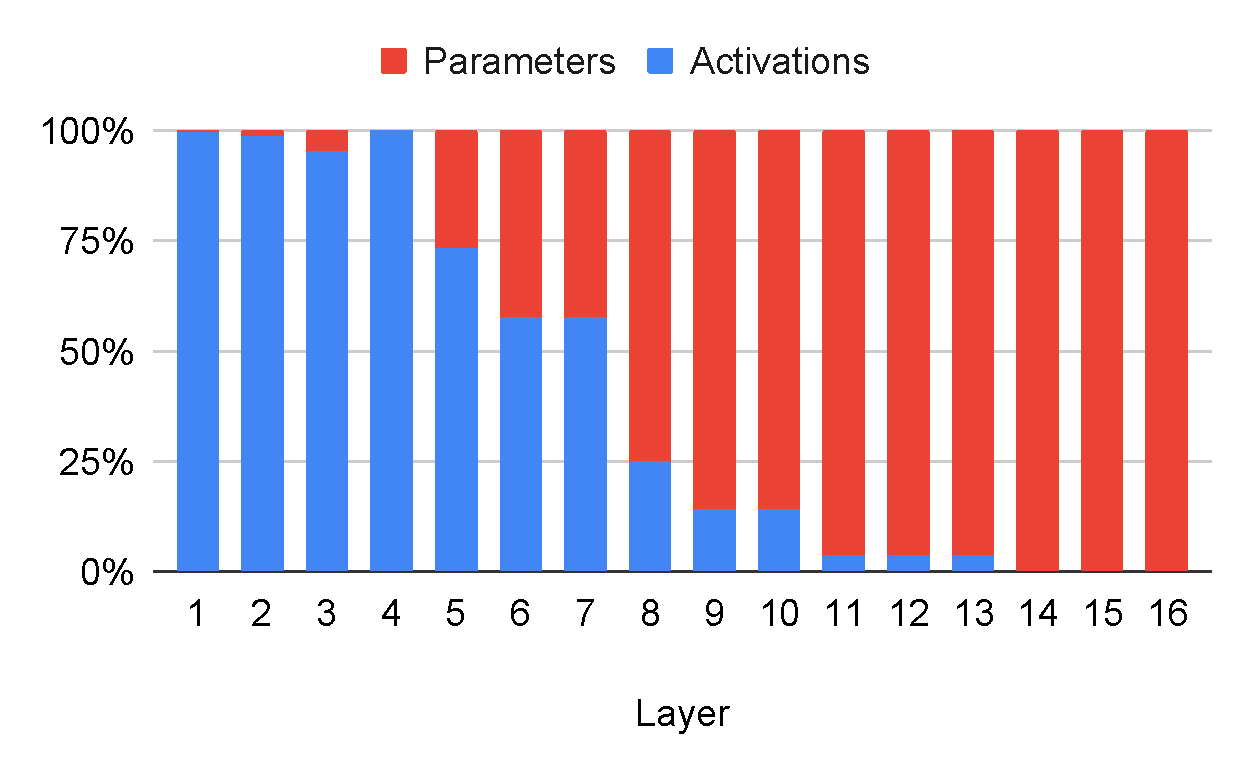
\includegraphics[width=0.49\textwidth]{VGG16ParamsNActivations}
		\label{fig:VGG16ParamsNActivations}}
	\hfil	
	\subfloat[AlexNet]{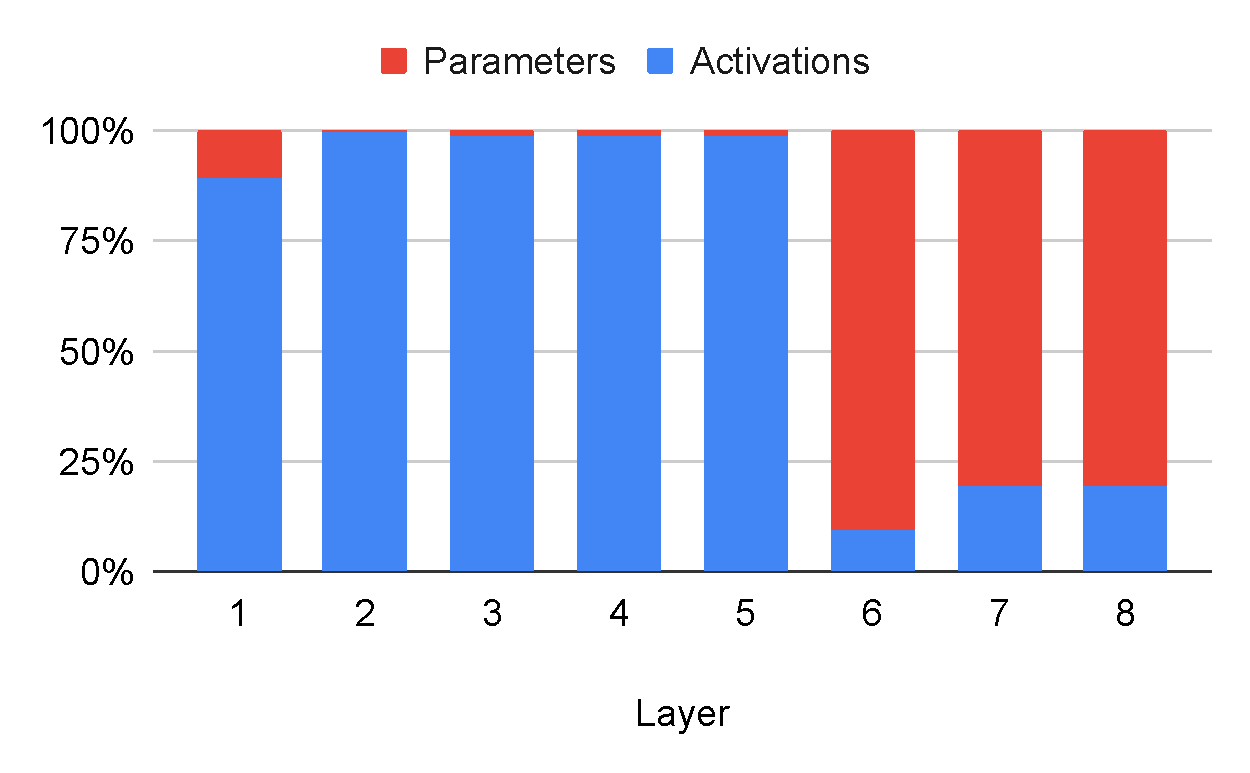
\includegraphics[width=0.49\textwidth]{AlexNetParamsNact.pdf}
		\label{fig:AlexNetParamsNact}}
	\hfil	
	\caption{Parameters and activations proportions in CL and FC layers of CNNs.}
	\label{fig:ParamsNactProp}
\end{figure}
\section{Related Work}
Zhang et al.~\cite{zhang2015optimizing} used loop tiling to optimize the off-chip memory accesses. They expressed the off-chip memory access as a function of tile dimensions and layer shape and determined optimal tile dimensions by enumerating all the legal tile dimensions. To reduce the hardware design complexity, they determined a global optimal tile dimension and used a common data reuse scheme for all the layers. Due to varying layer shapes, the optimal tile dimension and data-reuse scheme for different layers vary. Li et al.~\cite{Li2018SmartShuttleOO} proposed a layer-wise adaptive data partitioning and scheduling scheme to overcome this. However, their approach ignored the architectural parameters and address alignment and assumed that all tiles of the same dimensions have the same off-chip memory accesses. With this assumption, the tile dimensions determined by their approaches are suboptimal.
\section{Off-Chip Memory Accesses of CNN Layers}\label{MemAccess_CNN}
\subsection{Off-chip memory access of CL}\label{sec:AccessCLData}
A CNN accelerator accesses 3D data of \textit{ifm, ofm}, and \textit{wts} of each layer partitioned into tiles. It accesses tiles of the layer from off-chip memory one or multiple times. Trip counts of the tiles depend on the layer shape, tile dimensions, and the data reuse scheme. If the batch size is $D$, layer shape is $\langle W_o,H_o,N_i,M_o\rangle$ and tiling parameters are $\langle T_{c_o},T_{r_o},T_{n_i},T_{m_o}\rangle$, trip counts of tiles in IRO, ORO, and WRO schemes can be expressed as the rows of the matrix $\mathbf{R}$ in ~\eqref{eq:TripCount}, where columns represent \textit{ifm, ofm}, and \textit{wts} trip counts.
\begin{align}\label{eq:TripCount}
	\mathbf{R}=
	\begin{bmatrix}
		\mathbf{r}_{iro} \\  \mathbf{r}_{oro} \\ \mathbf{r}_{wro} \\
	\end{bmatrix}=
	\begin{bmatrix}
		D&(2\ceil[\big]{\frac{N_i}{T_{n_i}}}-1)D&\ceil[\big]{\frac{H_o}{T_{r_o}}}\ceil[\big]{\frac{W_o}{T_{c_o}}}D\\[6pt]
		\ceil[\big]{\frac{M_o}{T_{m_o}}}D&D&\ceil[\big]{\frac{H_o}{T_{r_o}}}\ceil[\big]{\frac{W_o}{T_{c_o}}} D\\[6pt]
		\ceil[\big]{\frac{M_o}{T_{m_o}}}D&(2\ceil[\big]{\frac{N_i}{T_{n_i}}}-1)D&1\\
	\end{bmatrix}
\end{align}
First we compute the off-chip memory accesses for one trip of each data type using Algorithm~\ref{Algorithm1} as below
\begin{align*}
	\begin{split}
		\numBytesOffChip_{ifm}=&\emph{BWA}(\addressSym_{ifm},\langle T_{c_i}, T_{r_i},T_{n_i}\rangle,\langle W_i,H_i,N_i\rangle,\numOverlap)\\
		\numBytesOffChip_{ofm}=&\emph{BWA}(\addressSym_{ofm},\langle T_{c_o},T_{r_o},T_{m_o}\rangle,\langle W_o,H_o,M_o\rangle,0)\\
		\numBytesOffChip_{wts}=&M_o\cdot \emph{BWA}(\addressSym_{wts},\langle K,K,T_{n_i}\rangle,\langle K,K,N_i\rangle,0)
	\end{split}
\end{align*} 
where $\numOverlap=(K-S)$ is the number of overlapping elements between adjacent $ifm$ tiles, $K$ is the filter size, and $S$ is the stride. $\numBytesOffChip_{ifm}$, $\numBytesOffChip_{ofm}$, and $\numBytesOffChip_{wts}$ are number of bytes accessed from off-chip memory for one trip of \textit{ifm, ofm} and \textit{wts} respectively. $\langle W_{i},H_{i},N_{i}\rangle$ are the \textit{ifm} data shape and $\langle T_{c_i},T_{r_i},T_{n_i}\rangle$ are the \textit{ifm} tile dimensions, which are related to \textit{ofm} layer shape and tile dimensions as below
\begin{align}\label{eq:ofmAndifmTileDims}
	\begin{split}
		H_o=(\frac{H_{i}+2\cdot P-K}{S}+1), ~\ &W_o=(\frac{W_{i}+2\cdot P-K}{S}+1)\\
		T_{r_o}=\frac{T_{r_{i}}-K}{S}+1,~\ &T_{c_o}=\frac{T_{c_{i}}-K}{S}+1
	\end{split}
\end{align}  
where $P$ is the padding. The total number of bytes accessed for j$^{th}$ reuse scheme ($\numBytesOffChip_j$) can be expressed as following sum
\begin{equation} \label{eq:TotalOffChipAccess}
	\numBytesOffChip_j=\mathbf{r_j}\cdot \begin{bmatrix}
		\numBytesOffChip_{ifm} &
		\numBytesOffChip_{ofm} &
		\numBytesOffChip_{wts}
	\end{bmatrix}^{T}
\end{equation}
where \textbf{r}$_j$ is the row vector of the matrix $\mathbf{R}$ for the j$^{th}$ scheme. 
\subsection{Optimization problem}
Now, we present determining the optimal tile dimensions as a constraint optimization problem. Tiles of \textit{ifm, ofm} and \textit{wts} reside in on-chip memory. Volume of the tiles is given by equation~\eqref{eq:tilesVol} below
\begin{align}\label{eq:tilesVol}
	\begin{bmatrix}
		V_i \\ V_o \\ V_w
	\end{bmatrix}=
	\begin{bmatrix}
		T_{c_i}\cdot T_{r_i}\cdot T_{n_i}\\
		T_{c_o}\cdot T_{r_o}\cdot T_{m_o}\\
		K^2\cdot T_{n_i}\cdot T_{m_o}\\
	\end{bmatrix}
\end{align}
where $V_i, V_o, \text{and }V_w$ are the sizes of \textit{ifm, ofm}, and \textit{wts} tiles, respectively. If the on-chip memory buffer size is $\BuffSize$ and each data element is represented by $\dataWidth$ bytes, then constraints on tile dimensions are
\begin{align}\label{eq:onChipConstraint}
	\begin{split}
		&(V_i + V_w + V_o)\cdot \dataWidth\leq \BuffSize \\
		&0<T_{c_o}\leq W_o,~\ 0<T_{r_o}\leq H_o\\
		&0<T_{n_i}\leq N_i,~\ 0<T_{m_o}\leq M_o
	\end{split}
\end{align}
Determining the tile dimensions which minimize the off-chip memory accesses, expressed by equation \eqref{eq:TotalOffChipAccess}, is a constraint optimization problem. The  number of bytes accessed from off-chip memory using j$^{th}$ reuse scheme $\numBytesOffChip_j$ (~\eqref{eq:TotalOffChipAccess}) and the constraints (~\eqref{eq:onChipConstraint}) are non-linear functions of four variables $\langle T_{c_o},T_{r_o},T_{n_i},T_{m_o}\rangle$, and thus solving it is non-trivial.
\subsection{Off-chip memory access of FCL}\label{sec:AccessFCLData}
The computations of FCLs are special case of CLs with  additional constraints on layer shapes and parameters. The \textit{ifm} volume is same as a filter volume i.e., $H_i{=}W_i{=}K$, padding $P{=}0$, and stride $S{=}1$. In CNNs, typical values of K are 1, 3, 5, 7 and 11. Due to small values of $H_i$ and $W_i$, these dimensions are not partitioned ($T_{r_i}{=}T_{c_i}{=}K$). \textit{ofm} layer shape and tile dimensions computed using ~\eqref{eq:ofmAndifmTileDims} are $\langle 1,1,M_o\rangle$ and $\langle 1,1,T_{m_o}\rangle$.

For FCLs, trips count of different data reuse schemes can be computed using equation~\ref{eq:TripCount}and the number of bytes accessed from off chip memory ($\numBytesOffChip^{FC}$) using~\eqref{eq:TotalOffChipAccess} by applying the layer shape constraints. The constraints on tile dimensions are given by~\eqref{eq:onChipConstraint}. $T_{n_i}$ and $T_{m_o}$ are the unknowns to be determined in~\eqref{eq:TotalOffChipAccess}. Determining the optimal tile dimensions for FCLs is a constraint optimization problem, similar to CL.
\section{Implementation and Results}
\subsection{Implementation}
The optimal tile dimensions can be determined by computing the number of bytes accessed from off-chip memory ($\numBytesOffChip$) at all the feasible points in the solution space. 
We have developed the model that computes $\numBytesOffChip$ of the CLs using the BWA approach (Algorithm~\ref{Algorithm1}) and finds the optimal tile dimensions. The tool also analyses the $\numBytesOffChip$ for different data reuse schemes to suggest the best scheme for each CL. It can be configured for different on-chip memory sizes, bus widths, and data bit width. It took less than 60 minutes to determine the optimal solution for VGG16 on Intel Core i7-6700 CPU (@3.40GHz$\times$8).
\subsection{Validation}\label{Validation}
We have validated the number of bytes accessed from off-chip memory computed by BWA (Algorithm~\ref{Algorithm1}) using the Xilinx tools. Our validation code is implemented using the Xilinx SDSoC framework, SDx v2018.3, which generates hardware functions from high-level languages like C/C++. We used the SDx pragmas to use zero\_copy as a data mover. The Xilinx tools provide the option to integrate the AXI Performance Monitor (APM) IP~\cite{APM}, which captures the real-time performance metrics like bus latency, amount of memory traffic for connected AXI interfaces. The target platform is ZedBoard, working at 100MHz frequency and off-chip memory (DRAM) is accessed using 64 bits AXI bus. 
Our validation code takes the 3D shape, and tile dimensions as input and the generated hardware functions access the 3D data from DRAM using loop tiling. The integrated APM IP logs the number of bytes and latency of off-chip memory access transactions using which we validated the number of bytes accessed from off-chip memory computed by our approach for different 3D data shapes and tile dimensions.
\subsection{Benchmarks}
We carried out experiments on three popular CNN networks, VGG16~\cite{simonyan2014very}, AlexNet~\cite{krizhevsky2012imagenet}, and ResNet~\cite{he2016deep} having 8, 16, and 50 layers, respectively. These CNNs have varying shapes and use filters of dimensions $1{\times}1$, $3{\times}3$, $5{\times}5$, $7{\times}7$, and $11{\times}11$. To compare the results with other approaches, we have used the on-chip buffer size of 108 KB, batch size of 3 for VGG16, and 4 for ResNet and AlexNet, as used by Eyeriss~\cite{chen2016eyeriss} and SmartShuttle~\cite{Li2018SmartShuttleOO}. 
\subsection{Baselines}
We have implemented the SmartShuttle (SS)~\cite{Li2018SmartShuttleOO} approach  to compare the results with our bus width aware (BWA) approach. SS statically determines the partitioning and scheduling scheme for each layer. It performs better than strategies that use a fixed tile dimension and data reuse scheme for all layers, e.g., Eyeriss~\cite{chen2016eyeriss} and  Zhang~\cite{zhang2015optimizing}. 
\subsection{Results}
\begin{figure}[!t]
	\centering
	\subfloat[$\numBytesOffChip_{VGG16}$]
	{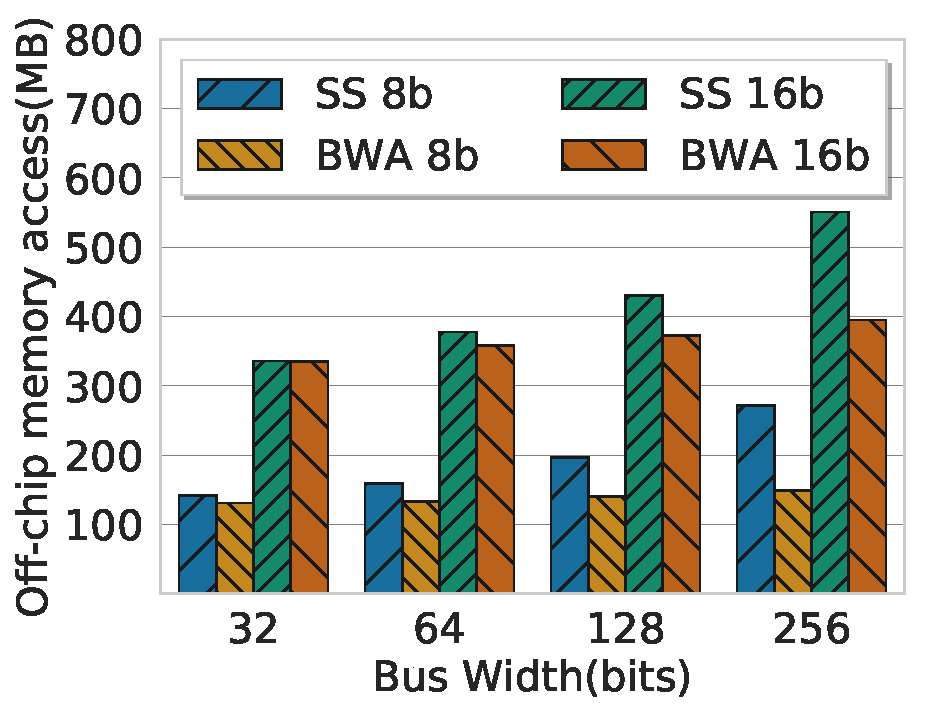
\includegraphics[width=0.32\textwidth]{VGG16_mem108_batch4_bw0_dW0_AD0.pdf}
		\label{fig:VGG16OffChipAccesses}}
	\hfil	
	\subfloat[$\numBytesOffChip_{AlexNet}$]
	{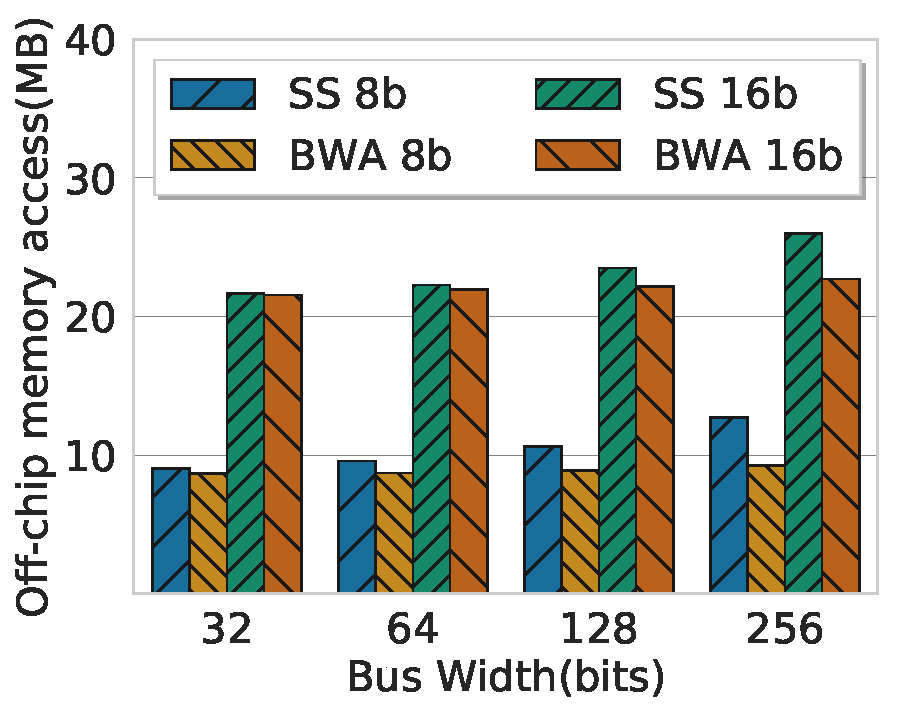
\includegraphics[width=.32\textwidth]{AlexN_mem108_batch4_bw0_dW0_AD0.pdf}
		\label{fig:AlexNetOffChipAccesses}}
	\hfil			
	\subfloat[$\numBytesOffChip_{ResNet}$]
	{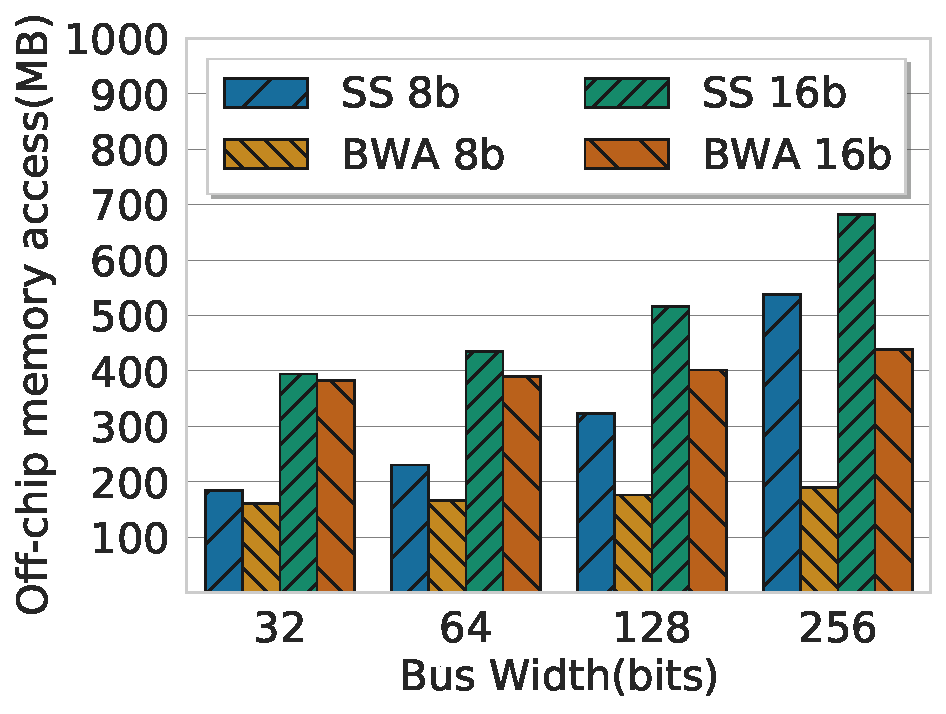
\includegraphics[width=.32\textwidth]{RESNet_mem108_batch4_bw0_dW0_AD0.pdf}
		\label{fig:ResNetOffChipAccesses}}
	\hfil	
	\caption{Off-chip memory access of convolution layers for 8 and 16 bits data width. BWA: Bus Width Aware, SS: SmartShuttle}
	\label{fig:AccessenOn64BitDataBus}
	\vspace{-1.0em}
\end{figure}
\subsubsection{Impact of Bus Width on memory access of CLs}
Fig.~\ref{fig:AccessenOn64BitDataBus} shows the number of bytes accessed from off-chip memory ($\numBytesOffChip$) of CLs of the CNNs for different bus widths for 8 and 16 bits data width and 108 KB on-chip buffer size. For a wider data bus, $\numBytesOffChip$ is more. BWA approach reduces the impact of bus-width on off-chip memory accesses, as it selects the tile dimensions considering the bus width and address alignments. Whereas, tile dimensions selected by SS remains the same, irrespective of bus width of the accelerator, which results in a large value of $\numBytesOffChip$.
As shown in Fig.~\ref{fig:AccessenOn64BitDataBus}, BWA reduces $\numBytesOffChip$ compared to SS for the three CNNs. For ResNet:50 it reduces $\numBytesOffChip_{ResNet}$ by 13\%, 28\%, 46\%, and 65\% for 8 bits data width and by 10\%, 22\% and 36\% for 16 bits data width on 64, 128, and 256 bits wide data bus, respectively, compared to SS. 
BWA reduces $\numBytesOffChip_{VGG16}$ by 8\%, 16\%, 29\%, and 45\% and $\numBytesOffChip_{AlexNet}$ by 4\%, 9\%, 16\% and 27\% on 32, 64, 128, and 256 bits wide buses respectively, for 8 bits data width. 
The impact of bus width is significant when accessing low-resolution data on a wide data bus. For 16 bits data width, the effectiveness of the BWA approach is noticeable for 64 or wider data buses. For 16 bits data width, BWA reduces $\numBytesOffChip_{VGG16}$ by 5\%, 13.5\% and 28\% and $\numBytesOffChip_{AlexNet}$ by 1.5\%, 5.7\% and 13\% compared to SS on 64, 128, and 256 bits wide data bus, respectively.
\subsubsection{Off-Chip Memory Access of Data Reuse  Schemes}\label{sec:ResultsDataReuseScheme}
\begin{figure}[htb]
	\centering
	\subfloat[VGG16 CLs]
	{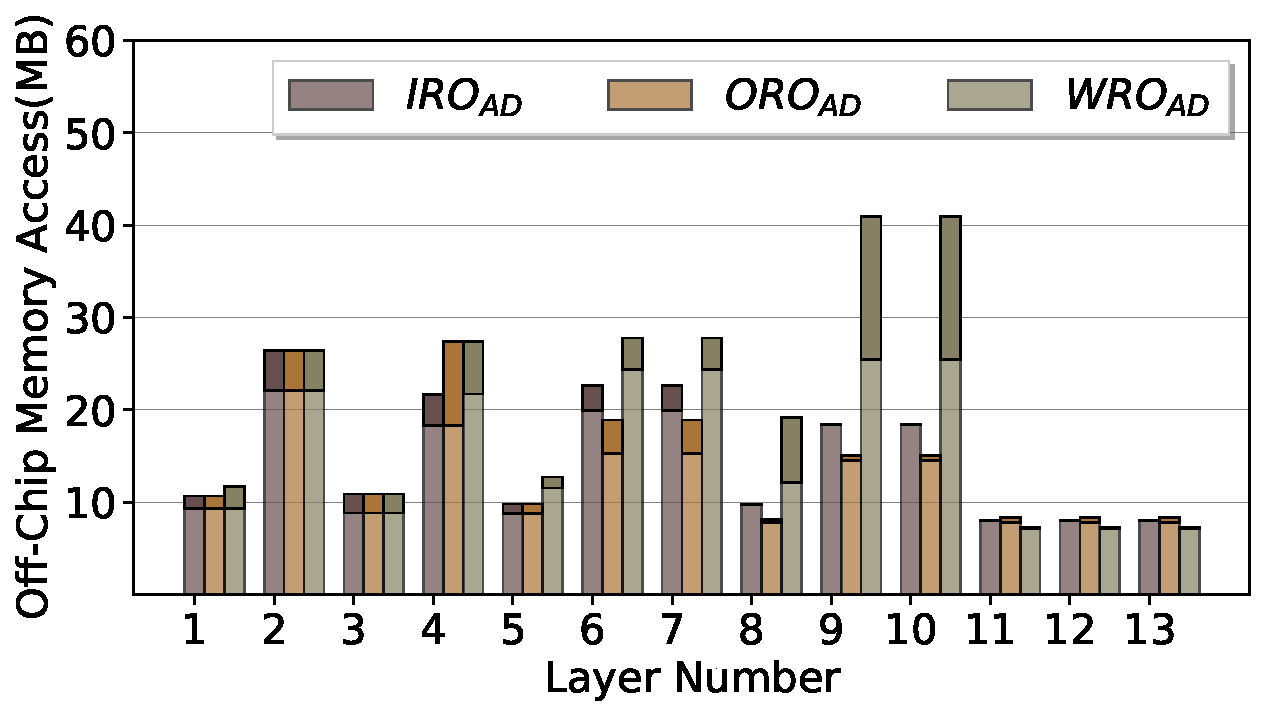
\includegraphics[width=0.45\textwidth]{VGG16_mem108_batch3_bw8_8bits_reuseSch.pdf}
		\label{fig:VGG16ReuseSchCompare}}
	\hfil
	\subfloat[AlexNet CLs]
	{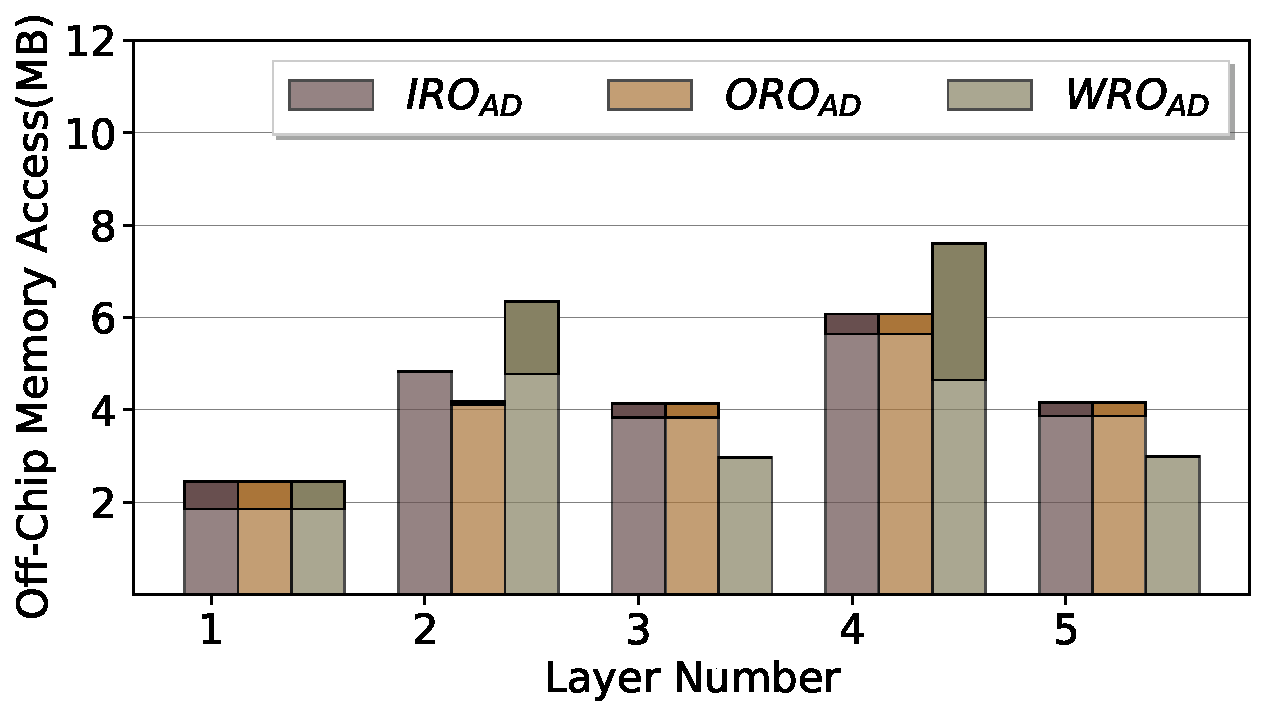
\includegraphics[width=0.45\textwidth]{AlexN_mem108_batch4_bw8_8bits_reuseSch.pdf}
		\label{fig:AlexNetReuseSchCompare}}
	\hfil	
	\caption{Layer wise off-chip memory access for IRO, ORO and WRO schemes.}
	\label{fig:DataReuseSchemeCompare}
	\vspace{-1.0em}	
\end{figure}
Figure~\ref{fig:DataReuseSchemeCompare} shows the layer-wise off-chip memory access of CLs of VGG16 and AlexNet for the three data reuse schemes using 64 bits wide bus and 8 bits data width. The results show that a single data reuse scheme is not optimal for all the layers. In the first few layers, IRO and ORO perform better than the WRO scheme, while in the last few layers, WRO outperforms the other two schemes. The solid color at the top of the bars shows the reduction in off-chip memory accesses when optimal tile dimensions are selected using the BWA approach compared to when tile dimensions are selected using the tile size-based approach. The BWA approach performs better than the tile size based approach for all the three data reuse schemes.
\subsubsection{On-chip Buffer Size}
\begin{figure}[htb]
	\centering
	\subfloat[$\numBytesOffChip_{VGG16}$]
	{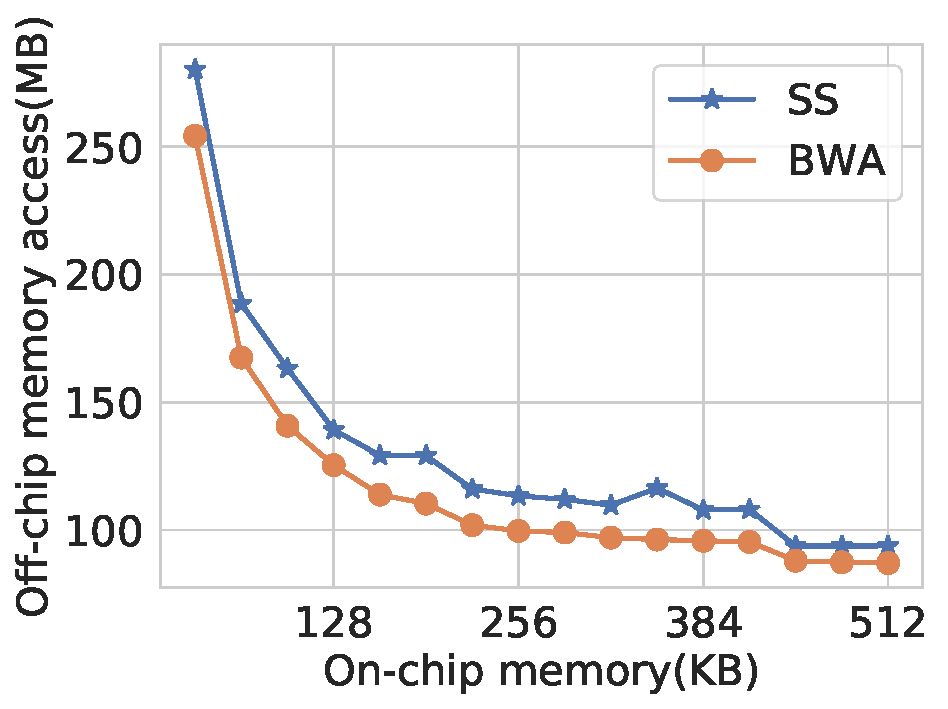
\includegraphics[width=0.42\textwidth]{VGG16_mem0_batch3_bw8_dW8_AD0.pdf}
		\label{fig:VGG16OnChipMemoryEffect}}
	\hfil
	\subfloat[$\numBytesOffChip_{AlexNet}$]
	{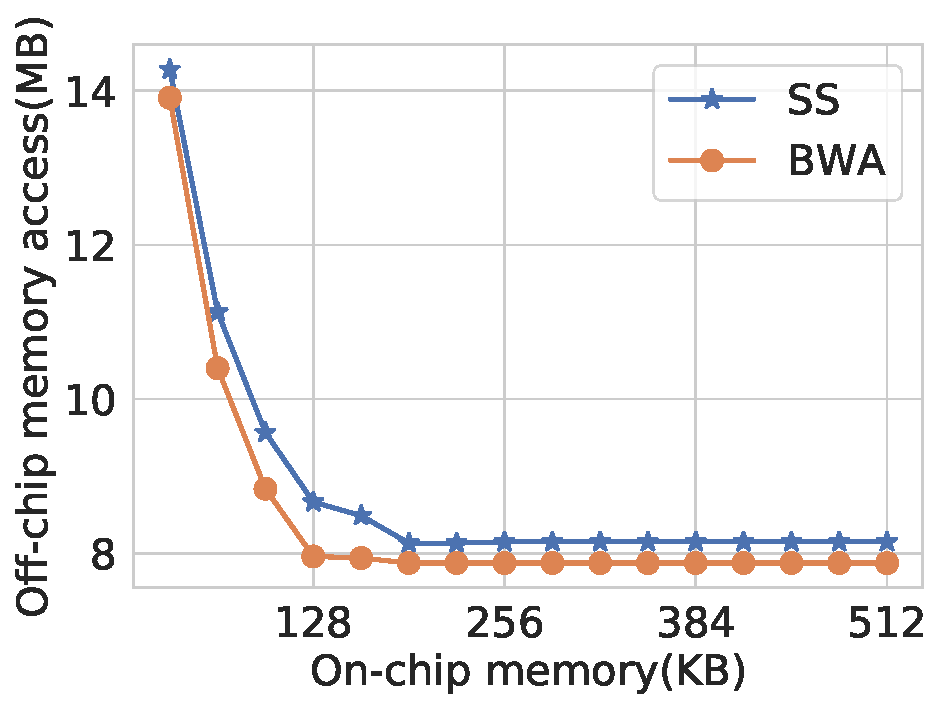
\includegraphics[width=0.42\textwidth]{AlexN_mem0_batch4_bw8_dW8_AD0.pdf}
		\label{fig:AlexNOnChipMemoryEffect}}
	\hfil
	\caption{Off-chip memory access for varying on-chip buffer sizes. BWA: Bus Width Aware, SS:SmartShuttle}
	\label{fig:EffectOfVaryingOnChipBuffer}
	\vspace{-1.0em}
\end{figure}
Fig.~\ref{fig:VGG16OnChipMemoryEffect} and Fig.~\ref{fig:AlexNOnChipMemoryEffect} compares the number of bytes accessed from off-chip memory ($\numBytesOffChip$) for different on-chip buffer sizes ($\BuffSize$) for VGG16 and AlexNet, respectively. Large on-chip buffer can accommodate larger tiles, which reduces the tiles trip counts (Equation~\ref{eq:TripCount}) and therefore the total off-chip memory accesses of the CNN (Equation~\ref{eq:TotalOffChipAccess}). This behavior is observed for both the CNNs in Fig.~\ref{fig:VGG16OnChipMemoryEffect} and Fig.~\ref{fig:AlexNOnChipMemoryEffect}. Both the approaches select the dimensions of the tiles  with the constraints of on-chip buffer size. However, the proposed BWA approach performs better as it considers the address alignments and bus width to reduce unwanted data transfers to optimizes the off-chip memory accesses, while SS approach ignores the architectural parameters.
\subsubsection{Impact of Bus Width on $\numBytesOffChip$ of FCLs}
\begin{figure}[htb]
	\centering
	\subfloat[VGG16]
	{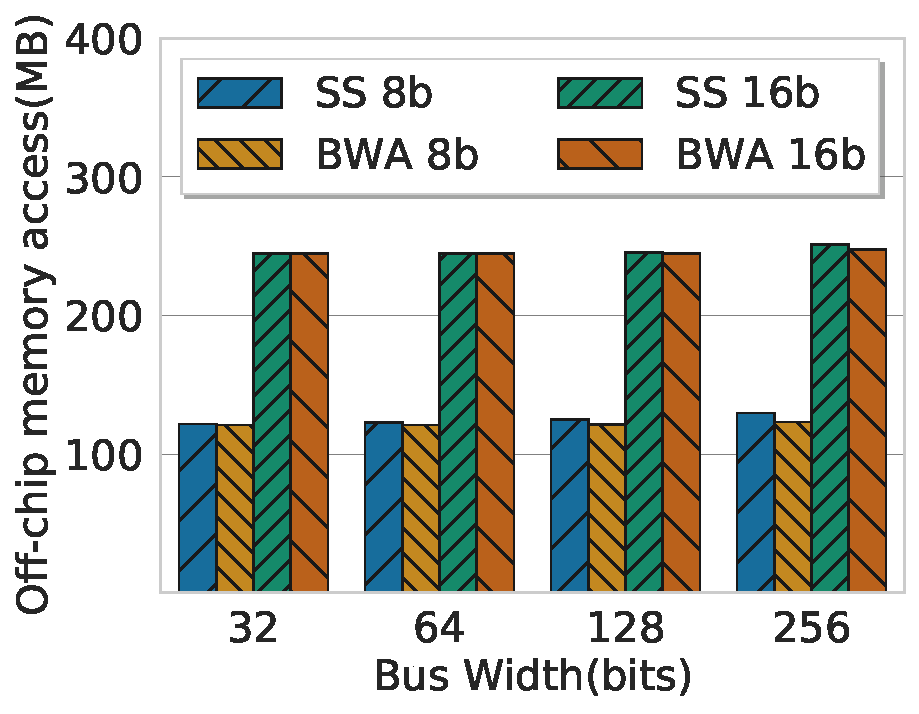
\includegraphics[width=0.4\textwidth]{VGG16_mem108_batch3_bw0_dW0_AD0_FC.pdf}
		\label{fig:VGG16FCLayer}}
	\hfil
	\subfloat[AlexNet]
	{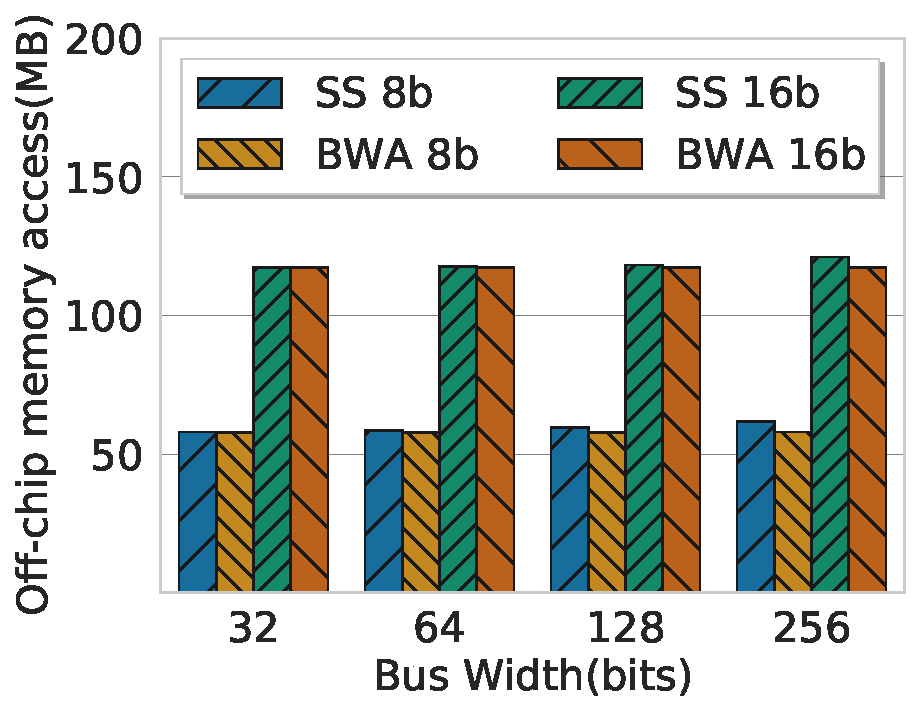
\includegraphics[width=0.4\textwidth]{AlexN_mem108_batch4_bw0_dW0_AD0_FC.pdf}
		\label{fig:AlexNetFCLayer}}
	\hfil	
	\caption{Off-chip memory access of Fully connected layers. BWA: Bus Width Aware, SS:SmartShuttle}
	\label{fig:EffectOnFC}
	\vspace{-1.0em}
\end{figure}
In FCLs, the height and width of tiles and data are the same. Tiles in FCL can be accessed from off-chip memory using a single transaction which results in fewer transactions in FCLs compared to CLs. Whereas in CLs, multiple transactions are required to access different rows of the tiles. Thus the impact of bus width is less on $\numBytesOffChip$ of FCLs as compared to CLs. \figurename~\ref{fig:VGG16FCLayer} and \figurename~\ref{fig:AlexNetFCLayer} shows the off-chip memory accesses of FCLs of VGG16 and AlexNet, respectively, for 8 bits data width. BWA reduces $\numBytesOffChip_{VGG16}^{FC}$ by 1\%, 2\%, 3\%, and 4\% and $\numBytesOffChip_{AlexNet}^{FC}$ by 0.2\%, 1\%, 3\% and 6\% on 32, 64, 128, and 256 bits wide buses, respectively.
\subsubsection{Latency And Energy Analysis}
\begin{figure}[htb]
	\centering
	\subfloat[VGG16]
	{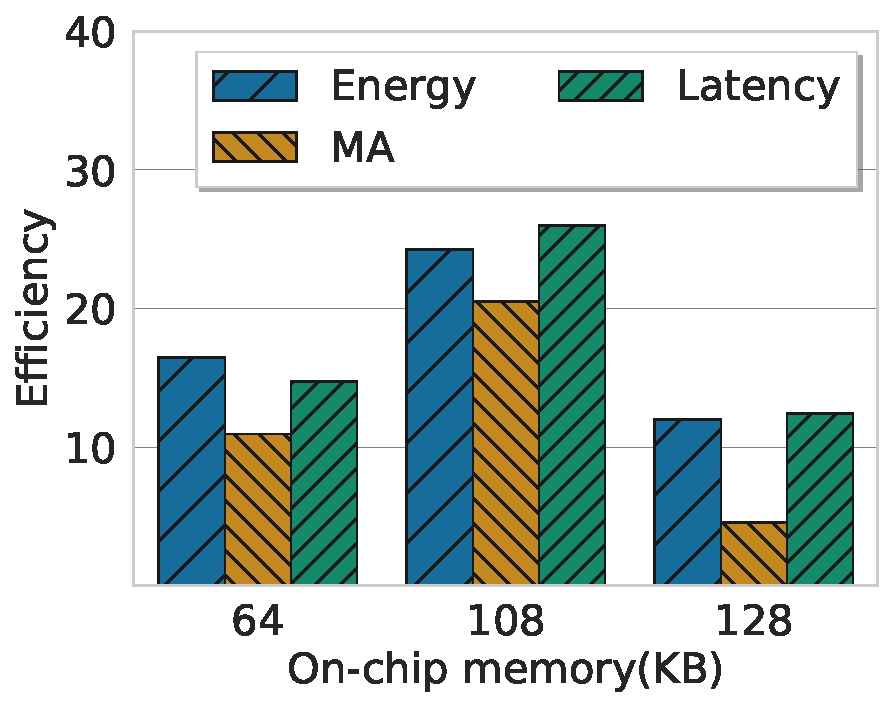
\includegraphics[width=0.4\textwidth]{energy_VGG16_DW8_BW64.pdf}
		\label{fig:VGG16EnergyEfficiency}}
	\hfil
	\subfloat[AlexNet]
	{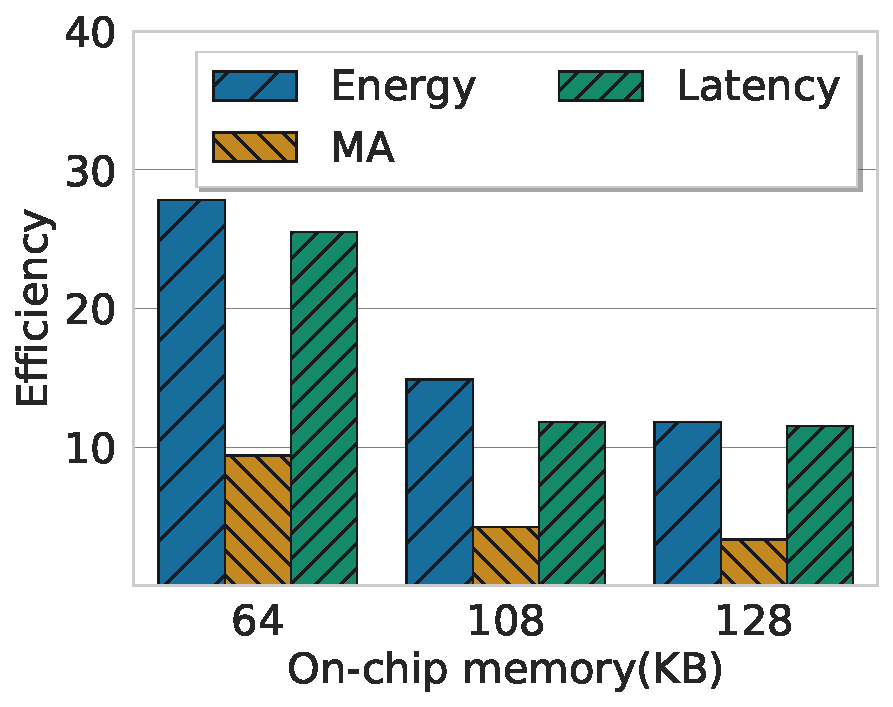
\includegraphics[width=0.4\textwidth]{energy_Alex_DW8_BW64.pdf}
		\label{fig:AlexEnergyEfficiency}}
	\hfil
	\caption{Energy and latency efficiency. BWA: Bus Width Aware, SS:SmartShuttle}
	\label{fig:EffectOnLatency}
	\vspace{-1.0em}
\end{figure}
Using our FPGA implementation, we measured the memory access latencies and execution time for CLs for the optimal tile dimensions determined using the approach described in~\ref{MemAccess_CNN}. To estimate the energy efficiency achieved by the BWA compared to the SS approach, we computed the energy consumption using the following equation~\cite{tu2017deep}
\begin{align}\label{eq:energyEfficiency}
	E~{=}~P\cdot Time~{+}~\numBytesOffChip\cdot E_{DDR}
\end{align}
where $P$ is the FPGA design power reported by the Vivado synthesis tool, $Time$ is the execution time, $\numBytesOffChip$ is the number of bytes accessed from off-chip memory logged using Xilinx APM IP, and $E_{DDR}$ is the off-chip memory access energy per bit. We have used $E_{DDR}$=70 pJ/bit, a typical value for the DDR3 memory access energy~\cite{6237004}.

\figurename{~\ref{fig:VGG16EnergyEfficiency}} and \figurename{~\ref{fig:AlexEnergyEfficiency}} show the energy, off-chip memory accesses, and latency efficiency achieved using the BWA compared to the SS approach for VGG16 and AlexNet, respectively, for 8 bits data width and 64 bits bus width. We observed that the changes in energy and latency are proportional to the changes in memory access. This observation confirms that off-chip memory access dominates the energy consumption of the CNN accelerators. 
\section{Summary}
Off-chip memory accesses dominate the energy consumption of CNN accelerators. Loop tiling is a common technique to partition the layer data into smaller tiles that fit into on-chip memory. The tile dimensions have a significant impact on the off-chip memory accesses of these accelerators. In this work, we propose a bus width and address alignment aware approach to compute the off-chip memory accesses of 3D data. Our tool statically analyses the memory accesses to find the optimal tile dimensions for CNN accelerators. Experimental results show that our approach reduces off-chip memory accesses of the CLs of VGG16 by 16\%, 29\%, and of AlexNet by 9\%, 16\% on 64, and 128 bits data bus respectively for 8 bits data width, compared to the state of the art approach.